\documentclass[11pt]{article}

% some definitions for the title page
\newcommand{\reporttitle}{Deep learning for GPU poor}
\newcommand{\reportdescription}{}

% load some definitions and default packages
%---------------------------------------------------------------------------
%	PACKAGES AND OTHER DOCUMENT CONFIGURATIONS
%---------------------------------------------------------------------------

\usepackage[twoside]{fancyhdr}
\usepackage{csquotes}

\usepackage[a4paper,hmargin=2.0cm,vmargin=1.0cm,includeheadfoot]{geometry}
% \usepackage{natbib} % for bibliography
\usepackage{biblatex}
\usepackage{tabularx,longtable,multirow,subfigure,caption}%hangcaption
\usepackage{fancyhdr} % page layout
\usepackage{url} % URLs
\usepackage[english]{babel}
\usepackage{graphicx}
\usepackage{rotating}
\usepackage{dsfont}
\usepackage{epstopdf} % automatically replace .eps with .pdf in graphics
% \usepackage{backref} % needed for citations
\usepackage{array}
\usepackage{latexsym}
\usepackage[pdftex,hypertexnames=false,colorlinks]{hyperref} % provide links in pdf (had pagebackref)
\usepackage{booktabs}
\usepackage{wrapfig}
\usepackage{caption}  % Required for \captionof
\usepackage{float} % for H option in figures
\usepackage{amssymb}
\usepackage{amsmath}
\usepackage{amsthm}
\usepackage{mathtools} % for 'dcases*' env.
\usepackage[nottoc]{tocbibind}

%%% Default fonts
\renewcommand*{\rmdefault}{bch}
\renewcommand*{\ttdefault}{cmtt}

%%% Default settings (page layout)
\setlength{\parindent}{0em}  % indentation of paragraph
\setlength{\parskip}{.3em}
\setlength{\itemsep}{0.mm}

\setlength{\headheight}{14.5pt}
\pagestyle{fancy}

\fancyfoot[ER,OL]{\thepage}%Page no. in the left on odd pages and on right on even pages

\fancyfoot[OC,EC]{\sffamily }
\renewcommand{\headrulewidth}{0.1pt}
\renewcommand{\footrulewidth}{0.1pt}
\captionsetup{margin=10pt,font=small,labelfont=bf}

% LISTINGS ammendments
\usepackage{listings}
\usepackage{color}

\definecolor{mygreen}{rgb}{0,0.6,0}
\definecolor{mygray}{rgb}{0.5,0.5,0.5}
\definecolor{mymauve}{rgb}{0.58,0,0.82}

\lstset{ 
  postbreak=\mbox{\textcolor{red}{$\hookrightarrow$}\space},
  backgroundcolor=\color{white},   % choose the background color; you must add \usepackage{color} or \usepackage{xcolor}; should come as last argument
  basicstyle=\footnotesize,        % the size of the fonts that are used for the code
  breakatwhitespace=false,         % sets if automatic breaks should only happen at whitespace
  breaklines=true,                 % sets automatic line breaking
  captionpos=b,                    % sets the caption-position to bottom
  commentstyle=\color{mygreen},    % comment style
%   deletekeywords={...},            % if you want to delete keywords from the given language
%   escapeinside={\%*}{*)},          % if you want to add LaTeX within your code
  extendedchars=true,              % lets you use non-ASCII characters; for 8-bits encodings only, does not work with UTF-8
  firstnumber=1,                % start line enumeration with line 1000
  frame=single,	                   % adds a frame around the code
  keepspaces=true,                 % keeps spaces in text, useful for keeping indentation of code (possibly needs columns=flexible)
  columns=fullflexible,
  keywordstyle=\color{blue},       % keyword style
  language=python,                 % the language of the code
  % morekeywords={*,...},            % if you want to add more keywords to the set
  numbers=left,                    % where to put the line-numbers; possible values are (none, left, right)
  numbersep=5pt,                   % how far the line-numbers are from the code
  numberstyle=\tiny\color{mygray}, % the style that is used for the line-numbers
  rulecolor=\color{black},         % if not set, the frame-color may be changed on line-breaks within not-black text (e.g. comments (green here))
  showspaces=false,                % show spaces everywhere adding particular underscores; it overrides 'showstringspaces'
  showstringspaces=false,          % underline spaces within strings only
  showtabs=false,                  % show tabs within strings adding particular underscores
  stepnumber=1,                    % the step between two line-numbers. If it's 1, each line will be numbered
  stringstyle=\color{mymauve},     % string literal style
  tabsize=2,	                   % sets default tabsize to 2 spaces
  title=\lstname% show the filename of files included with \lstinputlisting; also try caption instead of title
}

% Here, you can define your own macros. Some examples are given below.

\newcommand{\R}[0]{\mathds{R}} % real numbers
\newcommand{\Z}[0]{\mathds{Z}} % integers
\newcommand{\N}[0]{\mathds{N}} % natural numbers
\newcommand{\C}[0]{\mathds{C}} % complex numbers
\renewcommand{\vec}[1]{{\boldsymbol{{#1}}}} % vector
\newcommand{\mat}[1]{{\boldsymbol{{#1}}}} % matrix


%\bibliography{bibliography}

\begin{document}

% Include the title page
\begin{titlepage}

    \newcommand{\HRule}{\rule{\linewidth}{0.5mm}} % Defines a new command for the horizontal lines, change thickness here
    
    \center % Center everything on the page
     
    %------------------------------------------------------------------------
    %	HEADING SECTIONS
    %------------------------------------------------------------------------
    
    \textsc{\Large Department of Computing}\\[0.5cm] 
    \textsc{\large Imperial College of Science, Technology and Medicine}\\[0.5cm] 
    
    %------------------------------------------------------------------------
    %	TITLE SECTION
    %------------------------------------------------------------------------
    
    \HRule \\[0.4cm]
    { \huge \bfseries \reporttitle}\\ % Title of your document
    \HRule \\[0.4cm]

    \textit{\reportdescription}
    
    \vspace{2em}

    %------------------------------------------------------------------------
    %	AUTHOR SECTION
    %------------------------------------------------------------------------
    
    \large \emph{Author: Anton Zhitomirskiy}

    \vspace{1em}

    \global\let\newpagegood\newpage
    \global\let\newpage\relax
    
\end{titlepage}

\global\let\newpage\newpagegood

\tableofcontents

\clearpage

\section{Calculating statistics of a model}

\subsection{Foundation model parameter count}

Commonly when you look online for models, you will see their parameter counts. \emph{Transformers are typically described by the \#parameters} which impacts the computational requirements to store and run these models.

\subsection{Floating Point System}

\begin{figure}[H]
    \centering
    \subfigure{\fbox{
\includegraphics[page=4, trim=0cm 0cm 0cm 0cm, clip, width=.45\linewidth]{L15_deeplearning_for_gpu_poor_part_1.pdf}}}
    \subfigure{\fbox{
\includegraphics[page=5, trim=0cm 0cm 0cm 0cm, clip, width=.45\linewidth]{L15_deeplearning_for_gpu_poor_part_1.pdf}}}
    \caption{We store data in computers in bits with transistors. The more bits, the more precision.}
\end{figure}    



\begin{minipage}[l]{.5\linewidth}
    \begin{figure}[H]
        \centering
        \subfigure{\fbox{
\includegraphics[page=6, trim=0cm 0cm 0cm 0cm, clip, width=.95\linewidth]{L15_deeplearning_for_gpu_poor_part_1.pdf}}}
    \end{figure}    
\end{minipage}\hfill
\begin{minipage}[r]{.48\linewidth}
    \begin{itemize}
        \item \textbf{Floating point} is a way to represent numbers in a computer where the decimal point can float.
        \item A certain section is allocated to represent the precision (actual number) the exponent and the sign.
        \item still has the problem of underflow or overflow.
    \end{itemize}
\end{minipage}

\begin{minipage}[l]{.5\linewidth}
    \begin{figure}[H]
        \centering
        \subfigure{\fbox{
\includegraphics[page=7, trim=0cm 0cm 0cm 0cm, clip, width=.95\linewidth]{L15_deeplearning_for_gpu_poor_part_1.pdf}}}
    \end{figure}    
\end{minipage}\hfill
\begin{minipage}[r]{.48\linewidth}
    \begin{itemize}
        \item At inference time, just to store the data it is already 260GB
        \item At training time, we also require gradients and optimiser values (momentum, etc) which can be 10x the size of the model and the activations.
    \end{itemize}
\end{minipage}

\begin{minipage}[l]{.5\linewidth}
    \begin{figure}[H]
        \centering
        \subfigure{\fbox{
\includegraphics[page=8, trim=0cm 0cm 0cm 0cm, clip, width=.95\linewidth]{L15_deeplearning_for_gpu_poor_part_1.pdf}}}
    \end{figure}    
\end{minipage}\hfill
\begin{minipage}[r]{.48\linewidth}
    So if we pass through the network, we need to store the inputs to every single layer that theres a change in the computational graph. Here:
    \begin{itemize}
        \item The first is the batch times the number of tokens or the number of patches times by that dimensionality.
        \item For the query key value, they all get the same value.
        \item The attention matrix requires query with key-values
        \item We also need to store the $n^2$ complexity of the attention matrix. 
    \end{itemize}
\end{minipage}

\begin{itemize}
    \item Also we store the result of the soft max which is the batch times the number of heads times the sequence dimension.
    \item With multi-head attention we usually have another layer that learns how to combine these values together.
    \item All in all, we have 250GB for a batch size of 1. 
\end{itemize}

\begin{figure}[H]
    \centering
    \subfigure{\fbox{
\includegraphics[page=9, trim=0cm 0cm 0cm 0cm, clip, width=.45\linewidth]{L15_deeplearning_for_gpu_poor_part_1.pdf}}}
\end{figure}

\subsection{Floating Point Operations (FLOPs)}

\begin{minipage}[l]{.5\linewidth}
    \begin{figure}[H]
        \centering
        \subfigure{\fbox{
\includegraphics[page=10, trim=0cm 0cm 0cm 0cm, clip, width=.95\linewidth]{L15_deeplearning_for_gpu_poor_part_1.pdf}}}
    \end{figure}    
\end{minipage}\hfill
\begin{minipage}[r]{.48\linewidth}
    Computational requirements:
    \begin{itemize}
        \item given two vectors, if we add this will reuqire $n$ operations.
        \item For the dot products, there is $2n$ flops.
        \item For the matrix multiplication, there is $2nmp$ multiplications
    \end{itemize}
\end{minipage}

\begin{figure}[H]
    \centering
    \subfigure{\fbox{
\includegraphics[page=11, trim=0cm 0cm 0cm 0cm, clip, width=.95\linewidth]{L15_deeplearning_for_gpu_poor_part_1.pdf}}}
\end{figure}    

\begin{enumerate}
    \item the layer norm is roughly 20 operations for every feature and token
    \item for the query key values we have it 3 times, and 2 becuase its a dot product.
    \item The softmax: for every single query we dot product it for every single value.
    \item projectino is same as query key values (but only 1)
\end{enumerate}

\section{Deep Learning At Scale}

\begin{minipage}[l]{.5\linewidth}
    \begin{figure}[H]
        \centering
        \subfigure{\fbox{
\includegraphics[page=12, trim=0cm 0cm 0cm 0cm, clip, width=.95\linewidth]{L15_deeplearning_for_gpu_poor_part_1.pdf}}}
    \end{figure}    
\end{minipage}\hfill
\begin{minipage}[r]{.48\linewidth}
    \begin{itemize}
        \item For deeplearning we need model data and compute.
        \item At scale, you can't train the model many times for hyper-parmaeter tuning. A single model may take many dollars to train just once.
    \end{itemize}
\end{minipage}

\begin{minipage}[l]{.5\linewidth}
    \begin{figure}[H]
        \centering
        \subfigure{\fbox{
\includegraphics[page=13, trim=0cm 0cm 0cm 0cm, clip, width=.95\linewidth]{L15_deeplearning_for_gpu_poor_part_1.pdf}}}
    \end{figure}    
\end{minipage}\hfill
\begin{minipage}[r]{.48\linewidth}
    ``When they have limitless compute and limitless datasets, they saw this really nice power law trend where it sticks very closely to the trend. This says that generally you can predict quite well, if you have limited compute and limited dataset size what loss you would get at the end.''
    The values here were proven to be wrong because the smaller models were not fully optimized; they used the same learning rate schedule as they did for the larger models. Therefore, the line was too steep.
\end{minipage}

\begin{minipage}[l]{.5\linewidth}
    \begin{figure}[H]
        \centering
        \subfigure{\fbox{
\includegraphics[page=14, trim=0cm 0cm 0cm 0cm, clip, width=.95\linewidth]{L15_deeplearning_for_gpu_poor_part_1.pdf}}}
    \end{figure}    
\end{minipage}\hfill
\begin{minipage}[r]{.48\linewidth}
    ``openAI published finidngs about colour representing the size of the model, and they fit for given flops and compute budgets which model gets the lowest loss.'' 
    Here, we see that chinchilla is favoured since it prefers the number of data points over the model size.
\end{minipage}

\begin{minipage}[l]{.5\linewidth}
    \begin{figure}[H]
        \centering
        \subfigure{\fbox{
\includegraphics[page=15, trim=0cm 0cm 0cm 0cm, clip, width=.95\linewidth]{L15_deeplearning_for_gpu_poor_part_1.pdf}}}
    \end{figure}    
\end{minipage}\hfill
\begin{minipage}[r]{.48\linewidth}
    Here we see that `deep learning has bene sovled'. ``This is showing that this happens in all modalities; these losses can just keep going until we get to super human performance.''

    \definition[Reducible Loss]{
        It is the actual loss - the irreductible loss, where irreducible loss is viewed as the true entropy of the data i.e. if I had a perfect fit of the data, what would be my loss even if I had a perfect fit?

        It can be viewed as the KL divergence between the mainfold of the dataspace and the manafold of the learnt model. 
    }
\end{minipage}

\begin{figure}[H]
    \centering
    \subfigure{\fbox{
\includegraphics[page=16, trim=0cm 0cm 0cm 0cm, clip, width=.95\linewidth]{L15_deeplearning_for_gpu_poor_part_1.pdf}}}
    \caption{SORA AI just used more compute!}
\end{figure}    


\begin{minipage}[l]{.5\linewidth}
    \begin{figure}[H]
        \centering
        \subfigure{\fbox{
\includegraphics[page=17, trim=0cm 0cm 0cm 0cm, clip, width=.95\linewidth]{L15_deeplearning_for_gpu_poor_part_1.pdf}}}
    \end{figure}    
\end{minipage}\hfill
\begin{minipage}[r]{.48\linewidth}
    ``When we plot all modalities the number of compute days vs the number of parameters for the optimal setting. There are correlation between what it is like to compute potimal size model for videa and for language model''
\end{minipage}

\begin{minipage}[l]{.5\linewidth}
    \begin{figure}[H]
        \centering
        \subfigure{\fbox{
\includegraphics[page=18, trim=0cm 0cm 0cm 0cm, clip, width=.95\linewidth]{L15_deeplearning_for_gpu_poor_part_1.pdf}}}
    \end{figure}    
\end{minipage}\hfill
\begin{minipage}[r]{.48\linewidth}
    \begin{itemize}
        \item if blue is state of the art and red is my implementation,
        \item then we can do a scaling analysis and conclude that since the curve is steeper then it may perform better at high levels of compute. 
    \end{itemize}
\end{minipage}

\section{Methods for reducing computational requirements}

\subsection{Gradient Accumulation}

\begin{minipage}[l]{.5\linewidth}
    \begin{figure}[H]
        \centering
        \subfigure{\fbox{
\includegraphics[page=19, trim=0cm 0cm 0cm 0cm, clip, width=.95\linewidth]{L15_deeplearning_for_gpu_poor_part_1.pdf}}}
    \end{figure}    
\end{minipage}\hfill
\begin{minipage}[r]{.48\linewidth}
    \begin{itemize}
        \item As we increase the batch size our computation requirements increase
        \item If we use 1 batch, this is just Stochastic Gradient Descent so you're approximating the true gradient with one sample; your loss will be jumping around wihtout convergence 
        \item \emph{accumulate the gradients without updating the optimizer, then when the mini-batch size times the number of cumulative gradient accumulation steps equals the target batch then we do the step in the loss surface.}
        \item Useful if you want a larger batch size
    \end{itemize}
\end{minipage}

\subsection{Gradient Checkpointing}

\begin{minipage}[l]{.5\linewidth}
    \begin{figure}[H]
        \centering
        \subfigure{\fbox{
\includegraphics[page=20, trim=0cm 0cm 0cm 0cm, clip, width=.95\linewidth]{L15_deeplearning_for_gpu_poor_part_1.pdf}}}
    \end{figure}    
\end{minipage}\hfill
\begin{minipage}[r]{.48\linewidth}
    \begin{itemize}
        \item idea is to initially throw out the activation in the forward pass after we've done it, but in the backpropogation step we redo the entire forward computation step.
        \item This is computationally expensive, but the memory requirements stay low; it doesn't scale with the number of layers.
        \item The forward pass is much faster than the backwards pass
        \item Therefore, we select checkpoints from which we continue the forward pass. 
    \end{itemize}
\end{minipage}

\begin{minipage}[l]{.5\linewidth}
    \begin{figure}[H]
        \centering
        \subfigure{\fbox{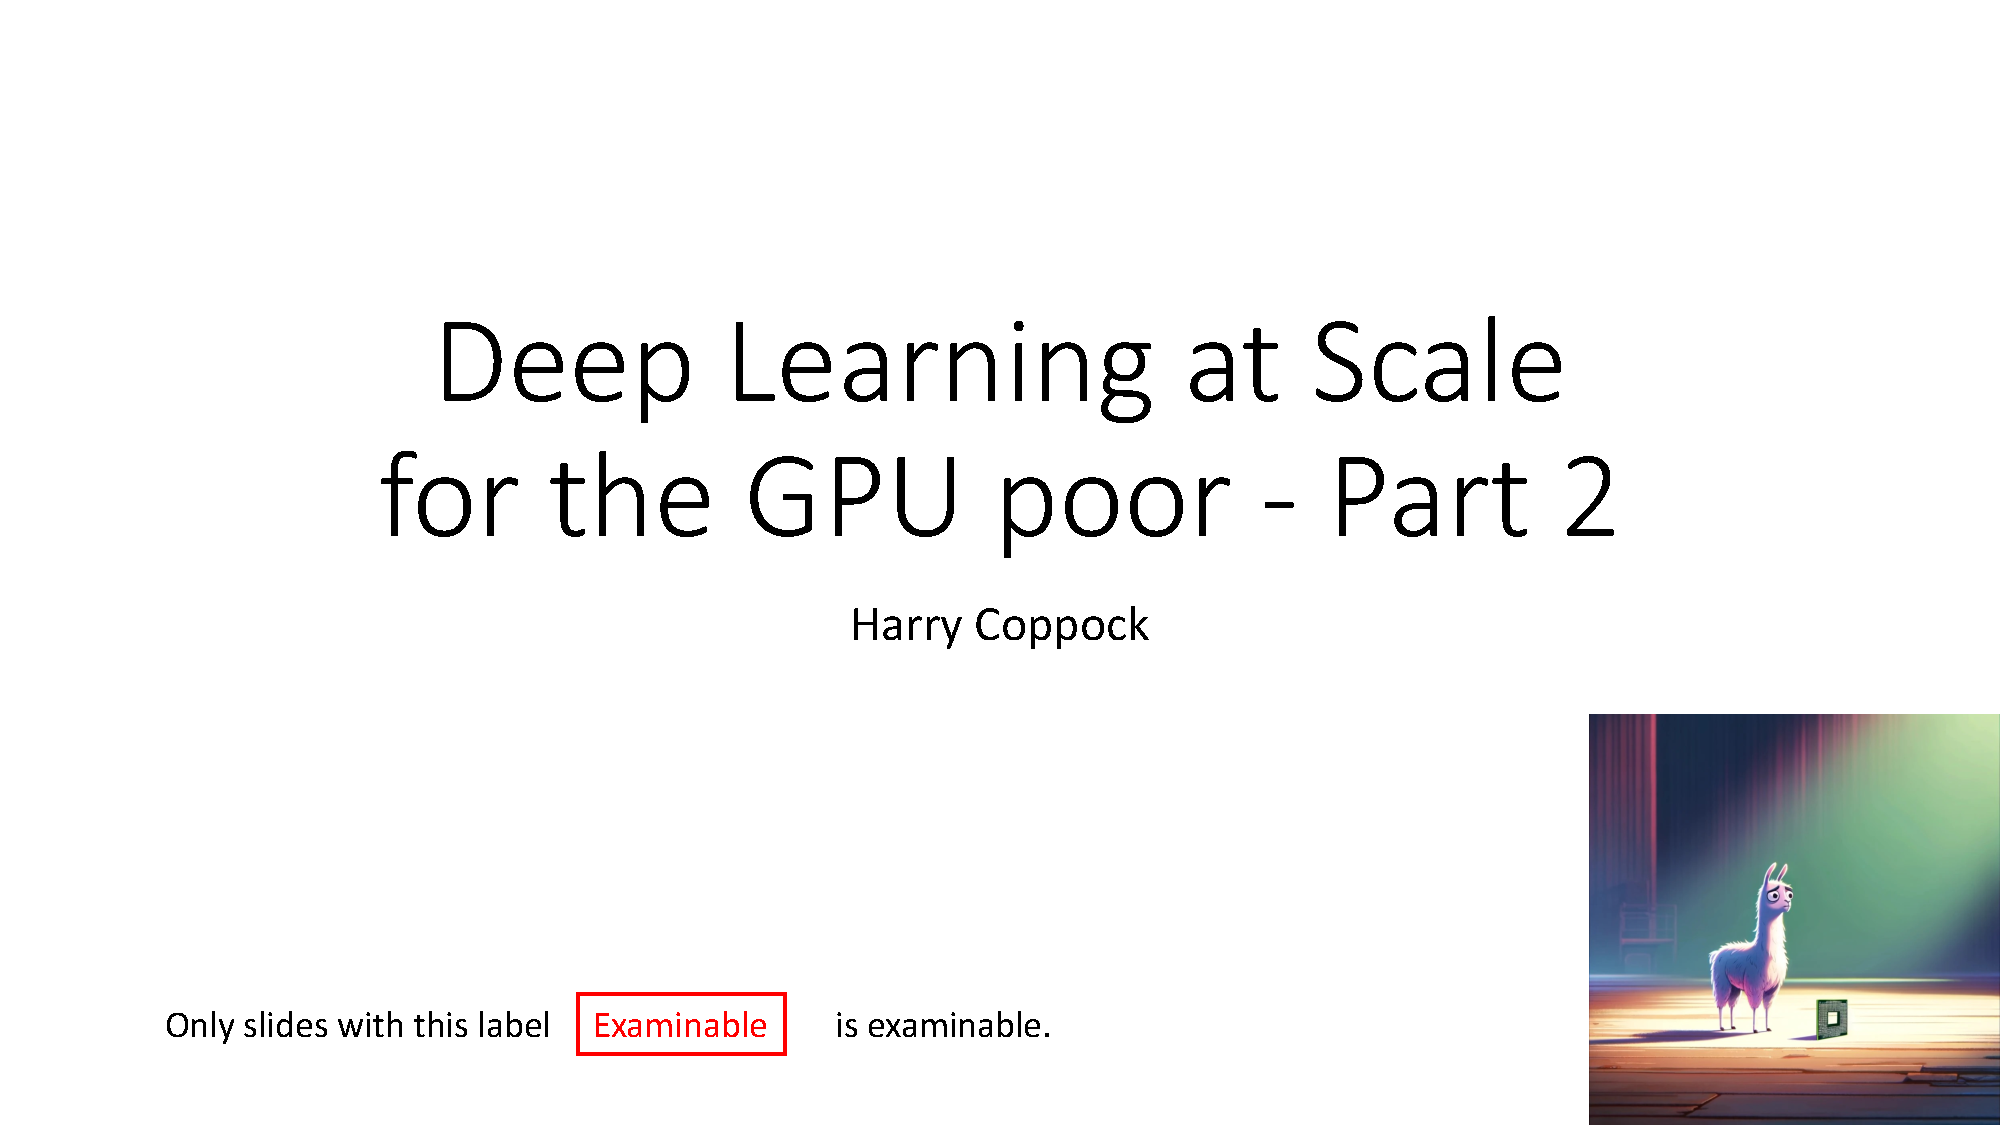
\includegraphics[page=1, trim=0cm 0cm 0cm 0cm, clip, width=.95\linewidth]{L16_deeplearning_at_scale_part2.pdf}}}
    \end{figure}    
\end{minipage}\hfill
\begin{minipage}[r]{.48\linewidth}
    \begin{itemize}
        \item
    \end{itemize}
\end{minipage}

\begin{minipage}[l]{.5\linewidth}
    \begin{figure}[H]
        \centering
        \subfigure{\fbox{\includegraphics[page=2, trim=0cm 0cm 0cm 0cm, clip, width=.95\linewidth]{L16_deeplearning_at_scale_part2.pdf}}}
    \end{figure}    
\end{minipage}\hfill
\begin{minipage}[r]{.48\linewidth}
    \begin{itemize}
        \item
    \end{itemize}
\end{minipage}

\begin{minipage}[l]{.5\linewidth}
    \begin{figure}[H]
        \centering
        \subfigure{\fbox{\includegraphics[page=3, trim=0cm 0cm 0cm 0cm, clip, width=.95\linewidth]{L16_deeplearning_at_scale_part2.pdf}}}
    \end{figure}    
\end{minipage}\hfill
\begin{minipage}[r]{.48\linewidth}
    \begin{itemize}
        \item
    \end{itemize}
\end{minipage}

\begin{minipage}[l]{.5\linewidth}
    \begin{figure}[H]
        \centering
        \subfigure{\fbox{\includegraphics[page=4, trim=0cm 0cm 0cm 0cm, clip, width=.95\linewidth]{L16_deeplearning_at_scale_part2.pdf}}}
    \end{figure}    
\end{minipage}\hfill
\begin{minipage}[r]{.48\linewidth}
    \begin{itemize}
        \item
    \end{itemize}
\end{minipage}

\begin{minipage}[l]{.5\linewidth}
    \begin{figure}[H]
        \centering
        \subfigure{\fbox{\includegraphics[page=5, trim=0cm 0cm 0cm 0cm, clip, width=.95\linewidth]{L16_deeplearning_at_scale_part2.pdf}}}
    \end{figure}    
\end{minipage}\hfill
\begin{minipage}[r]{.48\linewidth}
    \begin{itemize}
        \item
    \end{itemize}
\end{minipage}

\begin{minipage}[l]{.5\linewidth}
    \begin{figure}[H]
        \centering
        \subfigure{\fbox{\includegraphics[page=6, trim=0cm 0cm 0cm 0cm, clip, width=.95\linewidth]{L16_deeplearning_at_scale_part2.pdf}}}
    \end{figure}    
\end{minipage}\hfill
\begin{minipage}[r]{.48\linewidth}
    \begin{itemize}
        \item
    \end{itemize}
\end{minipage}

\begin{minipage}[l]{.5\linewidth}
    \begin{figure}[H]
        \centering
        \subfigure{\fbox{\includegraphics[page=7, trim=0cm 0cm 0cm 0cm, clip, width=.95\linewidth]{L16_deeplearning_at_scale_part2.pdf}}}
    \end{figure}    
\end{minipage}\hfill
\begin{minipage}[r]{.48\linewidth}
    \begin{itemize}
        \item
    \end{itemize}
\end{minipage}

\begin{minipage}[l]{.5\linewidth}
    \begin{figure}[H]
        \centering
        \subfigure{\fbox{\includegraphics[page=8, trim=0cm 0cm 0cm 0cm, clip, width=.95\linewidth]{L16_deeplearning_at_scale_part2.pdf}}}
    \end{figure}    
\end{minipage}\hfill
\begin{minipage}[r]{.48\linewidth}
    \begin{itemize}
        \item
    \end{itemize}
\end{minipage}

\begin{minipage}[l]{.5\linewidth}
    \begin{figure}[H]
        \centering
        \subfigure{\fbox{\includegraphics[page=9, trim=0cm 0cm 0cm 0cm, clip, width=.95\linewidth]{L16_deeplearning_at_scale_part2.pdf}}}
    \end{figure}    
\end{minipage}\hfill
\begin{minipage}[r]{.48\linewidth}
    \begin{itemize}
        \item
    \end{itemize}
\end{minipage}

\begin{minipage}[l]{.5\linewidth}
    \begin{figure}[H]
        \centering
        \subfigure{\fbox{\includegraphics[page=10, trim=0cm 0cm 0cm 0cm, clip, width=.95\linewidth]{L16_deeplearning_at_scale_part2.pdf}}}
    \end{figure}    
\end{minipage}\hfill
\begin{minipage}[r]{.48\linewidth}
    \begin{itemize}
        \item
    \end{itemize}
\end{minipage}

\begin{minipage}[l]{.5\linewidth}
    \begin{figure}[H]
        \centering
        \subfigure{\fbox{\includegraphics[page=11, trim=0cm 0cm 0cm 0cm, clip, width=.95\linewidth]{L16_deeplearning_at_scale_part2.pdf}}}
    \end{figure}    
\end{minipage}\hfill
\begin{minipage}[r]{.48\linewidth}
    \begin{itemize}
        \item
    \end{itemize}
\end{minipage}

\begin{minipage}[l]{.5\linewidth}
    \begin{figure}[H]
        \centering
        \subfigure{\fbox{\includegraphics[page=12, trim=0cm 0cm 0cm 0cm, clip, width=.95\linewidth]{L16_deeplearning_at_scale_part2.pdf}}}
    \end{figure}    
\end{minipage}\hfill
\begin{minipage}[r]{.48\linewidth}
    \begin{itemize}
        \item
    \end{itemize}
\end{minipage}

\begin{minipage}[l]{.5\linewidth}
    \begin{figure}[H]
        \centering
        \subfigure{\fbox{\includegraphics[page=13, trim=0cm 0cm 0cm 0cm, clip, width=.95\linewidth]{L16_deeplearning_at_scale_part2.pdf}}}
    \end{figure}    
\end{minipage}\hfill
\begin{minipage}[r]{.48\linewidth}
    \begin{itemize}
        \item
    \end{itemize}
\end{minipage}

\begin{minipage}[l]{.5\linewidth}
    \begin{figure}[H]
        \centering
        \subfigure{\fbox{\includegraphics[page=14, trim=0cm 0cm 0cm 0cm, clip, width=.95\linewidth]{L16_deeplearning_at_scale_part2.pdf}}}
    \end{figure}    
\end{minipage}\hfill
\begin{minipage}[r]{.48\linewidth}
    \begin{itemize}
        \item
    \end{itemize}
\end{minipage}

\begin{minipage}[l]{.5\linewidth}
    \begin{figure}[H]
        \centering
        \subfigure{\fbox{\includegraphics[page=15, trim=0cm 0cm 0cm 0cm, clip, width=.95\linewidth]{L16_deeplearning_at_scale_part2.pdf}}}
    \end{figure}    
\end{minipage}\hfill
\begin{minipage}[r]{.48\linewidth}
    \begin{itemize}
        \item
    \end{itemize}
\end{minipage}

\begin{minipage}[l]{.5\linewidth}
    \begin{figure}[H]
        \centering
        \subfigure{\fbox{\includegraphics[page=16, trim=0cm 0cm 0cm 0cm, clip, width=.95\linewidth]{L16_deeplearning_at_scale_part2.pdf}}}
    \end{figure}    
\end{minipage}\hfill
\begin{minipage}[r]{.48\linewidth}
    \begin{itemize}
        \item
    \end{itemize}
\end{minipage}

\begin{minipage}[l]{.5\linewidth}
    \begin{figure}[H]
        \centering
        \subfigure{\fbox{\includegraphics[page=17, trim=0cm 0cm 0cm 0cm, clip, width=.95\linewidth]{L16_deeplearning_at_scale_part2.pdf}}}
    \end{figure}    
\end{minipage}\hfill
\begin{minipage}[r]{.48\linewidth}
    \begin{itemize}
        \item
    \end{itemize}
\end{minipage}

\begin{minipage}[l]{.5\linewidth}
    \begin{figure}[H]
        \centering
        \subfigure{\fbox{\includegraphics[page=18, trim=0cm 0cm 0cm 0cm, clip, width=.95\linewidth]{L16_deeplearning_at_scale_part2.pdf}}}
    \end{figure}    
\end{minipage}\hfill
\begin{minipage}[r]{.48\linewidth}
    \begin{itemize}
        \item
    \end{itemize}
\end{minipage}

\begin{minipage}[l]{.5\linewidth}
    \begin{figure}[H]
        \centering
        \subfigure{\fbox{\includegraphics[page=19, trim=0cm 0cm 0cm 0cm, clip, width=.95\linewidth]{L16_deeplearning_at_scale_part2.pdf}}}
    \end{figure}    
\end{minipage}\hfill
\begin{minipage}[r]{.48\linewidth}
    \begin{itemize}
        \item
    \end{itemize}
\end{minipage}

\begin{minipage}[l]{.5\linewidth}
    \begin{figure}[H]
        \centering
        \subfigure{\fbox{\includegraphics[page=20, trim=0cm 0cm 0cm 0cm, clip, width=.95\linewidth]{L16_deeplearning_at_scale_part2.pdf}}}
    \end{figure}    
\end{minipage}\hfill
\begin{minipage}[r]{.48\linewidth}
    \begin{itemize}
        \item
    \end{itemize}
\end{minipage}

\begin{minipage}[l]{.5\linewidth}
    \begin{figure}[H]
        \centering
        \subfigure{\fbox{\includegraphics[page=21, trim=0cm 0cm 0cm 0cm, clip, width=.95\linewidth]{L16_deeplearning_at_scale_part2.pdf}}}
    \end{figure}    
\end{minipage}\hfill
\begin{minipage}[r]{.48\linewidth}
    \begin{itemize}
        \item
    \end{itemize}
\end{minipage}

\begin{minipage}[l]{.5\linewidth}
    \begin{figure}[H]
        \centering
        \subfigure{\fbox{\includegraphics[page=22, trim=0cm 0cm 0cm 0cm, clip, width=.95\linewidth]{L16_deeplearning_at_scale_part2.pdf}}}
    \end{figure}    
\end{minipage}\hfill
\begin{minipage}[r]{.48\linewidth}
    \begin{itemize}
        \item
    \end{itemize}
\end{minipage}

\begin{minipage}[l]{.5\linewidth}
    \begin{figure}[H]
        \centering
        \subfigure{\fbox{\includegraphics[page=23, trim=0cm 0cm 0cm 0cm, clip, width=.95\linewidth]{L16_deeplearning_at_scale_part2.pdf}}}
    \end{figure}    
\end{minipage}\hfill
\begin{minipage}[r]{.48\linewidth}
    \begin{itemize}
        \item
    \end{itemize}
\end{minipage}

\begin{minipage}[l]{.5\linewidth}
    \begin{figure}[H]
        \centering
        \subfigure{\fbox{\includegraphics[page=24, trim=0cm 0cm 0cm 0cm, clip, width=.95\linewidth]{L16_deeplearning_at_scale_part2.pdf}}}
    \end{figure}    
\end{minipage}\hfill
\begin{minipage}[r]{.48\linewidth}
    \begin{itemize}
        \item
    \end{itemize}
\end{minipage}

\begin{minipage}[l]{.5\linewidth}
    \begin{figure}[H]
        \centering
        \subfigure{\fbox{\includegraphics[page=25, trim=0cm 0cm 0cm 0cm, clip, width=.95\linewidth]{L16_deeplearning_at_scale_part2.pdf}}}
    \end{figure}    
\end{minipage}\hfill
\begin{minipage}[r]{.48\linewidth}
    \begin{itemize}
        \item
    \end{itemize}
\end{minipage}

\begin{minipage}[l]{.5\linewidth}
    \begin{figure}[H]
        \centering
        \subfigure{\fbox{\includegraphics[page=26, trim=0cm 0cm 0cm 0cm, clip, width=.95\linewidth]{L16_deeplearning_at_scale_part2.pdf}}}
    \end{figure}    
\end{minipage}\hfill
\begin{minipage}[r]{.48\linewidth}
    \begin{itemize}
        \item
    \end{itemize}
\end{minipage}

\begin{minipage}[l]{.5\linewidth}
    \begin{figure}[H]
        \centering
        \subfigure{\fbox{\includegraphics[page=27, trim=0cm 0cm 0cm 0cm, clip, width=.95\linewidth]{L16_deeplearning_at_scale_part2.pdf}}}
    \end{figure}    
\end{minipage}\hfill
\begin{minipage}[r]{.48\linewidth}
    \begin{itemize}
        \item
    \end{itemize}
\end{minipage}

\begin{minipage}[l]{.5\linewidth}
    \begin{figure}[H]
        \centering
        \subfigure{\fbox{\includegraphics[page=28, trim=0cm 0cm 0cm 0cm, clip, width=.95\linewidth]{L16_deeplearning_at_scale_part2.pdf}}}
    \end{figure}    
\end{minipage}\hfill
\begin{minipage}[r]{.48\linewidth}
    \begin{itemize}
        \item
    \end{itemize}
\end{minipage}

\begin{minipage}[l]{.5\linewidth}
    \begin{figure}[H]
        \centering
        \subfigure{\fbox{\includegraphics[page=29, trim=0cm 0cm 0cm 0cm, clip, width=.95\linewidth]{L16_deeplearning_at_scale_part2.pdf}}}
    \end{figure}    
\end{minipage}\hfill
\begin{minipage}[r]{.48\linewidth}
    \begin{itemize}
        \item
    \end{itemize}
\end{minipage}

\begin{minipage}[l]{.5\linewidth}
    \begin{figure}[H]
        \centering
        \subfigure{\fbox{\includegraphics[page=30, trim=0cm 0cm 0cm 0cm, clip, width=.95\linewidth]{L16_deeplearning_at_scale_part2.pdf}}}
    \end{figure}    
\end{minipage}\hfill
\begin{minipage}[r]{.48\linewidth}
    \begin{itemize}
        \item
    \end{itemize}
\end{minipage}

% \printbibliography
% \addcontentsline{toc}{section}{Bibliography}

\end{document}